\section{Methods}

\subsection{Experimental Setup}

All tests were conducted at RAMLAB's facilities at the port of Rotterdam's Innovation Dock. The robotic printer, as shown in \autoref{fig:robot_setup}, is their customized Techman XXX 6-axis robot with a Fronius TPS 320i CMT-capable MIG power source.
Atop the welding torch mount sits a RAMLAB-developed MaxQ system, capable of performing 3D scans of the workpiece to determine geometric printing accuracy, as well as thermal scans to determine the interpass temperature between layers. Some tests were performed before the thermal camera was calibrated, and thus a simple two-wire thermocouple was used.
Additionally, a Cavitar camera was used to record later tests to inspect the solidification process.

\begin{minipage}{\linewidth}
      \centering
      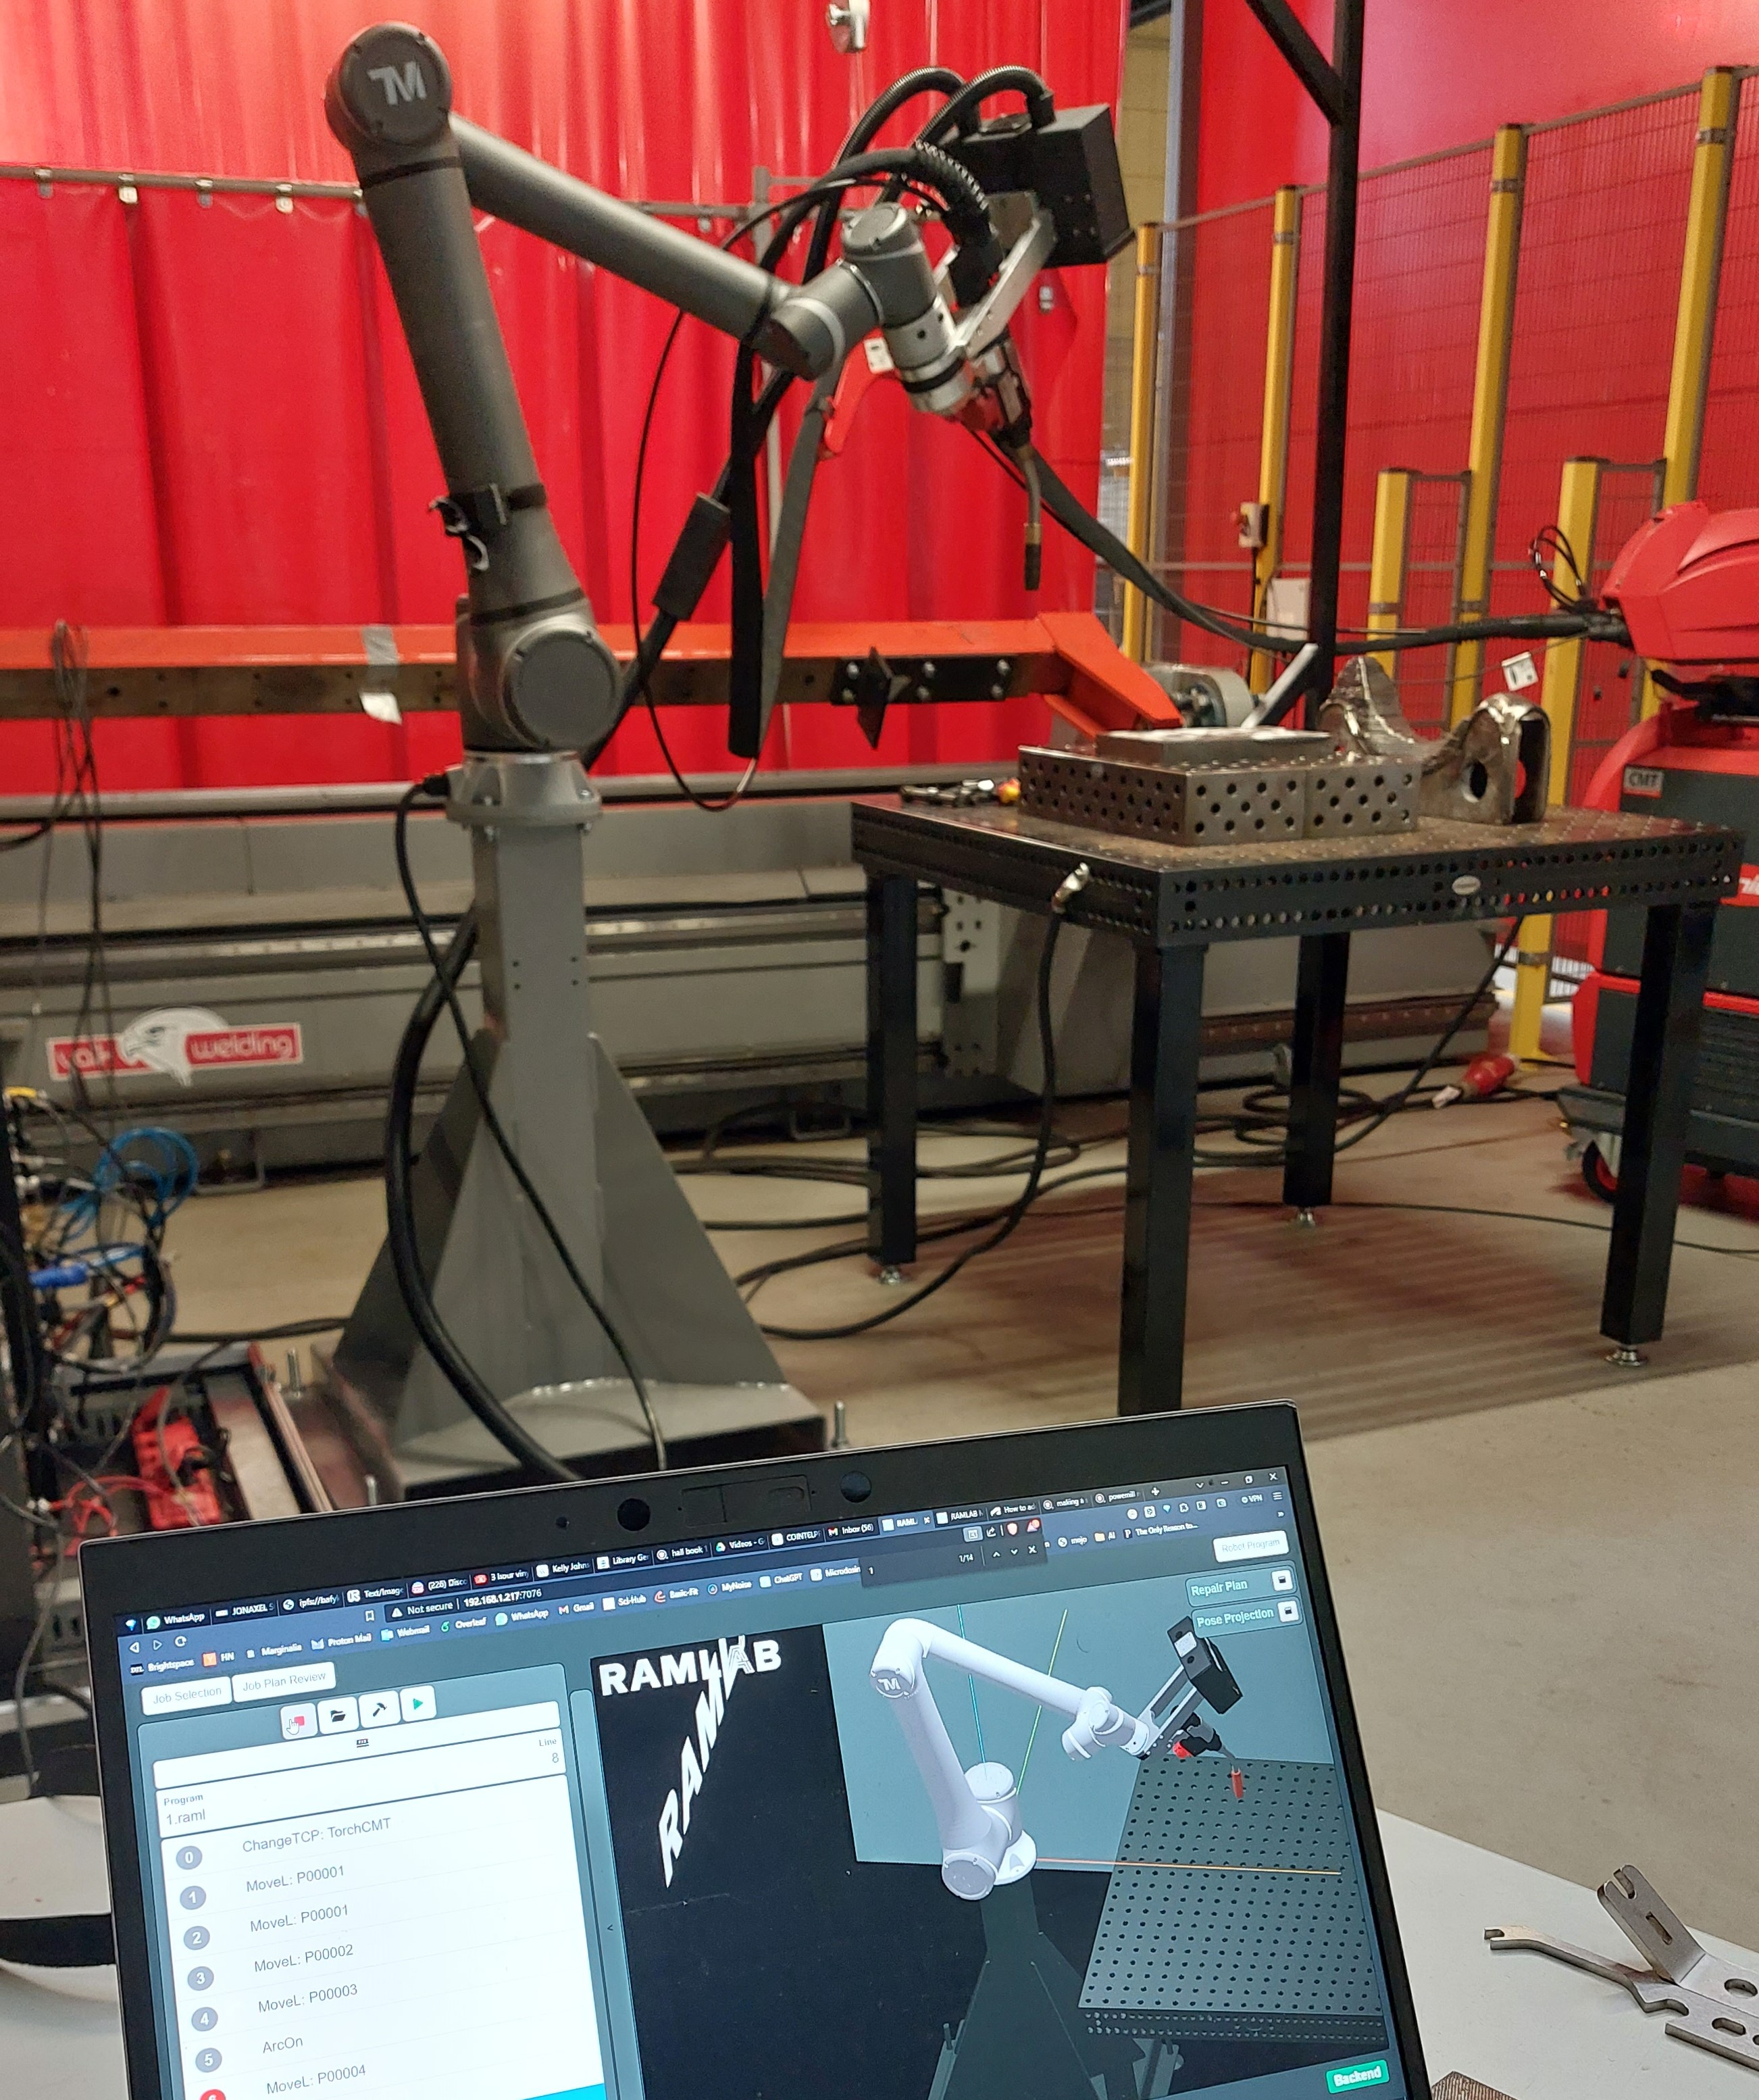
\includegraphics[width=\linewidth]{images/robot_setup.jpg}
      \captionof{figure}{Techman robot setup}
      \label{fig:robot_setup}
  \end{minipage}

The welds and geometries were created using Autodesk PowerShape and PowerMill and exported with RAMLAB's custom postprocessing software to make use of their MaxQ system.

The baseplates used were made of stainless steel with dimensions of 200x300x30 mm.

Because the Fronius power source does not yet have an experimental welder for the Fe-Co alloy, a welder program for a similar material was chosen. NiCrMo-3 has comparable atomic sizes to FeCo and also contains trace Molybdenum like Vacoflux 17, so it available welder program was chosen as a starting point. Because the Vacoflux 17 wire provided was 1 mm in diameter, the cladding (surface coating) preset was used, since it is optimized for lower deposition rates.

The shielding gas used was Alumaxx Plus X30S, composed of 30\% Helium and 70\% Argon, although the gas program used in the Fronius system was for pure Argon. The inclusion of Helium is important because of its high thermal conductivity, which disperses the arc energy, produces a wider and smoother arc, and allows for lower heat inputs and higher travel speeds. Combined with the use of CMT, this allows one to weld in significantly colder conditions than usual.

\subsection{Experimental Procedure}

The main objectives of this material characterization can be categorized as the following milestones:

\begin{enumerate}
    \item Minimum weldability for single beads
    \item Minimum weld quality for single beads and overlapping beads
    \item Minimum weld quality for single bead layers
    \item Process stability over many single-bead layers
    \item Minimum print quality for a full-scale part
    \item Magnetic and material property maintenance of samples and final part
\end{enumerate}

Instead of planning out all the experiments beforehand, the project was conducted in an iterative fashion, with each experiment informing the next. This was done to make the most of the limited time available and to ensure that the project would be able to reach the final milestone in the time available.

The process parameters were iteratively changed between welds, albeit with some limitations. The Fronius power source has feed rate/current/voltage relationships (called "welders") that have been experimentally determined for several materials, and these cannot be changed freely nor allow for independent control over the parameters. Because of this, only the feed rate was controlled for.

The process parameters that were altered for all welds were the following: feed rate, travel speed, SFI (Spatter Free Injection), arc length correction, initial current level (as a percentage of the main current) and initial current slope time.

The Spatter Free Injection by Fronius, also known as the Low Spatter Control (LSC) process, is a modified dip transfer arc welding process that achieves high-quality weld seams with minimal spattering and an increased deposition rate by triggering the short circuit at a low current level, leading to a gentle reignition and a stable welding process.

The arc length correction is a percentual correction of the distance between the tip of the wire and the workpiece, and since this distance is small, even small percentual changes can have an outsized effect. The initial current level is the percentage of the main current that is used for the initial arc ignition, and the initial current slope time is the time it takes for the current to ramp up to the main current level.

For overlapping beads, the spacing between beads was controlled. For layered single-bead walls, the layer height was taken as the running average of the wall, and the interpass temperature was controlled.







